\documentclass[12pt,a4paper]{report}
\usepackage[utf8]{inputenc}
\usepackage[T1]{fontenc}
	
\usepackage[francais]{babel}
\usepackage{lmodern}
\usepackage {textcomp}
\usepackage{amssymb}
\usepackage{mathrsfs}
\usepackage{amsmath}
\usepackage{amsfonts}

\usepackage{graphicx}
\usepackage{enumitem}
\usepackage{eurosym}
\usepackage[a4paper,left=2cm,right=2cm,top=2cm,bottom=2cm]{geometry}
\usepackage{hyperref}
\usepackage{gensymb}

\usepackage{listings,color}
\definecolor{verbgray}{gray}{0.9}
\setlength{\parskip}{1ex plus 0.5ex minus 0.2ex}
\newcommand{\hsp}{\hspace{20pt}}
\newcommand{\HRule}{\rule{\linewidth}{0.5mm}}
\renewcommand{\thesection}{\Alph{section}}
	
	\begin{document}
	
\begin{titlepage}
	\begin{sffamily}
		\begin{center}
			\begin{figure}
				
			\end{figure}
			
			\fbox{\textsc{\LARGE Projet PIC}}\\[1cm]
			
			\textsc{\Large Rapport final}\\[1.5cm]
			
			\HRule \\[0.4cm]
			{ \huge \bfseries Gestion d'un logiciel permettant la création, la mise à jour et la mise à disposition de l'usager des deux challenges "Swin \& run" et "Raid" propres à la fédération française de triathlon. \\[0.4cm] }
			\HRule \\[1.5cm]
			
			\centering{
				
\includegraphics[scale=1]{logo.png} 
			}\\[5cm]
			
			
			\begin{flushleft}
				Félix BOUTERAA \\
				Mohamed OULAAFFART \\
				Gaël SAGON \\
				2017-2018 \\
			\end{flushleft}  
			
			\begin{flushright}
				Mme. POISSON CAILLAULT
			\end{flushright}  
			
		\end{center}
	\end{sffamily}
\end{titlepage}

	
	\newpage
	
	\tableofcontents
	
	\newpage
	
	\listoffigures
	
	\newpage
	\addcontentsline{toc}{section}{Introduction}
	\section*{Introduction}
	Dans un contexte marqué par l’émergence du web, le besoin accru de l’informatisation et de l’automatisation des gestions, nous avons développé un site web pour permettre à la ligue des Hauts-de-France de mettre à jour les challenges organisés durant chaque année et aux participants de consulter leurs résultats.
	En effet, le long du processus de développement allant des premières phases de la définition des besoins fonctionnels du client jusqu’aux phases de création et de test, nous avons fixé trois lignes de conduite, à savoir :
	\begin{enumerate}
	\item Le site web doit satisfaire les besoins de ses utilisateurs et des administrateurs ;
	\item Il doit répondre aux qualités requises en matière de maintenabilité et de portabilité ;
	\end{enumerate}
	Afin de mettre la lumière sur les différentes démarches suivies pour l’aboutissement de ce travail, nous avons scindé ce rapport en trois grandes parties. Dans cette optique, la première sera réservée à l’illustration du contexte général du projet, tandis que la deuxième sera consacrée à l’étude analytique des différents processus de données et des phases de notre projet. Alors que la 3ème partie sera dédiée à la présentation des langages utilisés pour la réalisation du site web, de ses interfaces ainsi que des tests mis en œuvre pour s’assurer de son bon fonctionnement. Par ailleurs, il convient de préciser que ce rapport sera joint d’un guide d’utilisation qui sera mis à la disposition aux administrateurs de la ligue.
	\chapter{Context général du projet}
	Cette partie traitera du contexte général de notre projet d’Innovation et de Conception, en mettant l’accent essentiellement sur une brève présentation du maître d'ouvrage et de ses exigences fonctionnelles. Egalement, la méthodologie de travail adoptée ainsi que la planification du projet seront mises en avant.  
	
	\newpage
	\section {Context général du projet}
	\subsection{La ligue des Hauts-de-France du triathlon }
	
	La Ligue des Hauts-de-France de Triathlon est un organe décentralisé de la F.F.TRI. Elle est administrée par un Comité Directeur et un Bureau Directeur composés de membres élus en son sein. 
	Pour fonctionner, la ligue Hauts-de-France, a constitué plusieurs commissions dont chacune est présidée par un membre du Comité Directeur et composées de membres de la ligue volontaires et choisis pour leurs compétences.
	
	\subsection{Description du processus de l’organisation des challenges }
	L’organisateur de la course envoie les informations de tous les participants ainsi que leurs classements à la ligue. Ces fichiers sont envoyés sous formats PDF, Word, Tableurs Excel voire même papier.  Ces données sont envoyées à la ligue sans aucun traitement ou filtrage. Par conséquent, les administrateurs de la ligue ont pour première tâche de supprimer les participants qui ne sont pas inscrits au niveau de la ligue, et également de traiter le problème des homonymes d’une manière manuelle. Tâche qui demeure difficile et demande du temps.
	Une fois les données sont actualisées, les fichiers challenge sont mis à jour et les classements globaux sont établis. L’ensemble de ces opérations sont faites moyennant des fichiers Excel.
	
	
	\subsection{Les modalités du challenge  }
	Les challenges organisés sont soumis à plusieurs règles qui sont répertoriées comme suit :
	\begin{itemize} 
	\item 	Toutes les épreuves individuelles de cross duathlon, duathlon, aquathlon, cross triathlon et triathlon organisées par la Ligue NPdC, distance XS, S, M, L ou XL sont retenues pour le challenge.
	\item 	Les organisations s'inscrivant dans le circuit des épreuves du challenge doivent se soumettre au cahier des charges proposés par la Ligue.
	 \item  Seront retenues au challenge de l’année suivante uniquement les épreuves qui rempliront les contraintes et fourniront les résultats au format prévu au point 8 au plus tard dans la semaine suivant l’épreuve.
	
	\end{itemize} 
	 \paragraph	Attribution des points. Un classement individuel par catégorie et par sexe est réalisé à l’issue de chacune des épreuves. Seule la distance la plus longue accessible à la catégorie sera prise en compte dans l’obtention des points.
	L’attribution des points se fait en fonction du classement par catégorie et sexe. 
	
	Les tableaux figurant ci-dessous récapitulent le nombre de points attribués selon le classement du participant :
	\begin{enumerate}
	   \item Pour les adultes
	\begin{figure}[h!]
	   \center
	   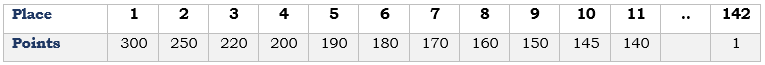
\includegraphics[scale=0.5]{points_categorie_adultes.png}
	   \caption {Les points attribués aux participants de la catégorie adultes selon leurs classements}
	\end{figure}
	
	Au-delà de la 142ème place, 1 point est attribué à chacun des participants. Les points obtenus sont pondérés par un coefficient dépendant de la distance de l’épreuve : 
	
	\begin{itemize} 
	 	\item 0,5 pour un XS ; 
	 	\item 0,75 pour un S ;
	 	\item  pour un M ; 
	 	\item 1,5 pour un L ;
	 	\item 2 pour un XL ou XXL.
	\end{itemize} 
	   \item Pour les jeunes
	\begin{figure}[!h]
	   \center
	   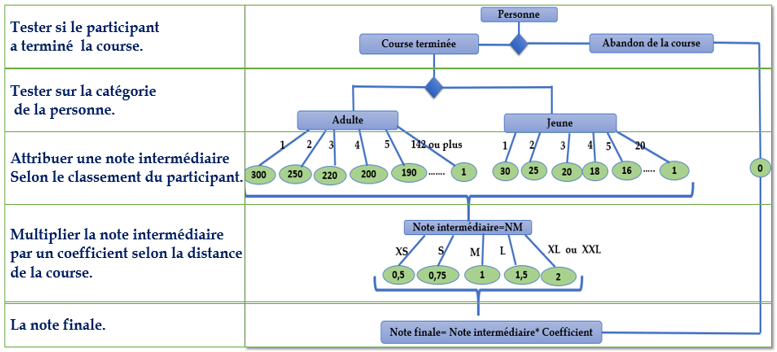
\includegraphics[scale=0.5]{points_categorie_jeunes.png}
	   \caption {Les points attribués aux participants de la catégorie jeunes selon leurs classements}
	\end{figure}
	
	\end{enumerate}
	Au-delà de la 20ème place, un point est attribué à chacun des participants. Les abandons et les absents ne marquent pas de point. 
	L’ensemble de ces règles susmentionnées sont récapitulées dans le schéma suivant :
	\begin{figure}
	   \center
	   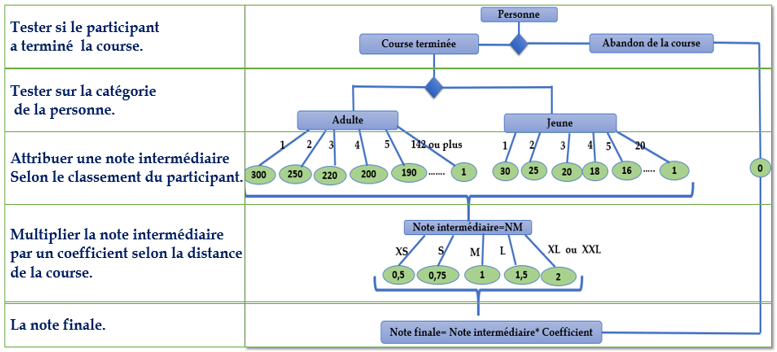
\includegraphics[scale=0.5]{recapitulatif_modalite_challenge.png}
	   \caption {Récapitulatif des modalités du challenge}
	\end{figure}
	
	\subsection{Expression des besoins fonctionnelles}
	L’outil développé dans le cadre de ce projet, doit répondre aux fonctionnalités définies en concertation avec le client lors des réunions. Ainsi l’ensemble de ces fonctionnalités sont répertoriées comme suit :
	\begin{itemize} 
	\item Supprimer les participants dans une courses et qui ne sont pas inscrits dans la ligue ;	
	\item Pallier au problème des homonymes ;
	\item Création d’un challenge
	\item La mise à jour d’un challenge ;
	\item Affichage des résultats globaux des courses ;
	\item Afficher les statiques individuels avec les graphes correspondants ;
	\item Effectuer des recherches des participants par plusieurs critères ;
	\item Toutes ces opérations doivent être réalisées émanant une interface graphique reluisante.
	\end{itemize} 
	
	\subsection {Méthodologie de travail }
	Afin de garantir la réussite du projet, il a été décidé de recourir à la méthodes agile SCRUM. En effet, celle-ci consiste à découper le projet en boites de temps appelées sprints. Chaque sprint commence par une estimation suivie d'une planification opérationnelle. Le sprint se termine par une démonstration de ce qui a été achevé. Avant de démarrer un nouveau sprint, l'équipe réalise une rétrospective. Cette technique analyse le déroulement du sprint achevé, afin d'améliorer ses pratiques. Le flot de travail de l'équipe de développement est facilité par son auto-organisation. 
	Pour mettre cette méthode en pratique. Une réunion est organisée chaque jeudi après-midi avec nos Encadrants pour discuter des avancements de la semaine en cours en de déterminer les tâches à effectuer durant la semaine à avenir. Par ailleurs, l’ensemble des tâches à réaliser sont répartis sur les membres de l’équipe afin de converger les efforts pour la réussite du projet. 
	
	
	\subsection{Diagramme de Gantt  }
	La planification est parmi les phases d’avant-projet. Elle consiste à prévoir le déroulement du projet tout au long de ses phases. Grâce aux réunions tenues avec nos encadrants et le client, on a été éclairés sur les différentes étapes du projet.
	Ainsi le diagramme ci-après résume les différentes étapes ainsi que le temps qui leurs a été allouée
	\begin{figure}
	   \center
	   \includegraphics[scale=0.5]{Diagramme_Gantt.png}
	   \caption {Le diagramme de Gantt du projet}
	\end{figure}
	
	
	\chapter{Etude analytique du projet}

Ce chapitre présentera les outils utilisés pour la réalisation de la conception de notre projet. Par ailleurs, il relate ses différentes étapes, ainsi que les diagrammes dégagés après chaque étape.
\section {Etude analytique du projet}


\subsection {Diagramme de packages }
\subsubsection{Définition}
Le diagramme de packages est un diagramme UML qui fournit une représentation graphique de haut niveau de l'organisation de l’application à réaliser.
\subsubsection{Diagramme de packages du projet}
De prime abord, il convient de distinguer les différents modules à développer dans le cadre du projet. Ainsi le diagramme de packages illustrer dans la figure ci-après montre clairement les trois modules à mettre en jeu.
\begin{figure}
	   \center
	   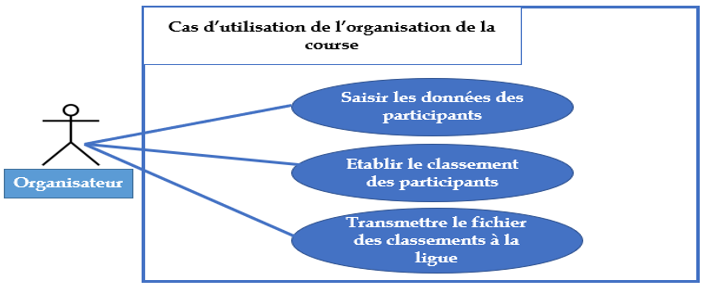
\includegraphics[scale=0.5]{Diagramme_de_packages.png}
	   \caption {Le diagramme de packages du projet}
\end{figure}

Ce diagramme permet de dégager trois packages principaux qui seront détaillés dans le cadre des cas d’utilisation illustré dans l’axe suivant.



\subsection {Les cas d’utilisation  }

\subsubsection{Définition}
Les cas d'utilisation sont définis par une description textuelle, décrivant les objectifs et interactions entre le système et ses acteurs. Le format de présentation textuelle des cas d'utilisation est libre.
\subsubsection{Diagramme de cas d’utilisation }
Comme illustré par le diagramme de packages, trois modules sont à développer. Ces modules nécessitent l’élaboration de trois cas d’utilisation. Le premier cas d’utilisation du projet traite de la phase de l’organisation d’une course (tel montré sur la figure ci-dessous). En effet le seul acteur qui interagit avec le système dans ce cas est l’organisateur de la course. Ainsi le système doit permettre de réaliser un certain nombre de fonctionnalités qui sont répertoriées comme suit :
\begin{itemize} 
\item La saisie des données des participants dans une course ;
\item  L’établissement du classement des participants dans la course ;
\item  L’envoi des résultats finaux à la ligue pour permettre à l’administrateur de mettre à jour le fichier des challenges.
\end{itemize} 

\begin{figure}
	   \center
	   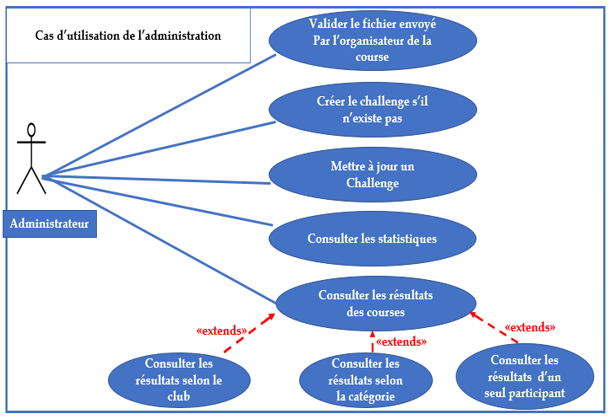
\includegraphics[scale=0.5]{Diagramme_cas_utilisation_organisation_course.png}
	   \caption {Le diagramme de cas d’utilisation relatif à l’organisation d’une course.}
\end{figure}


S’agissant de l’étape de l’administration, l’acteur qui utilise le système est l’administrateur de la ligue. Dans ce cas l’administrateur doit pouvoir effectuer les tâches suivantes :
\begin{itemize} 
\item Valider les fichiers des courses envoyé par les organisateurs des courses (Supprimer les participants qui ne sont pas inscrits dans la ligue, traiter les homonymes…) ;
\item Créer le fichier challenge, s’il n’existe pas et le mettre à jour ;
\item  Consulter les résultats et les statistiques inhérentes aux courses selon un certain nombre de critères de choix (comme les clubs, les catégories…).
\end{itemize} 
Ainsi la figues ci-desous  illustre clairement le cas d’utilisation de cette étape.



\begin{figure}
	   \center
	   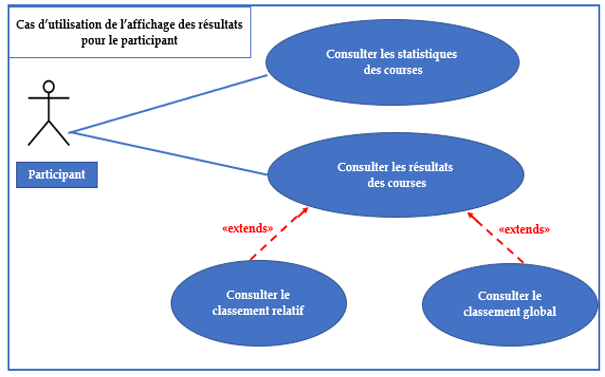
\includegraphics[scale=0.5]{Diagramme_cas_utilisation_administration_challenge.png}
	   \caption {Le diagramme de cas d’utilisation de la phase d’administration.}
\end{figure}
Le dernier cas d’utilisation concerne l’étape relative à l’affichage des résultats pour les sportifs.  Ainsi, le système devra permettre l’affichage des résultats globaux des courses, les classements relatifs et quelques graphes montrant l’évolution individuel pour chaque sportif.
La figure ci-après montre ces étapes :
\begin{figure}
	   \center
	   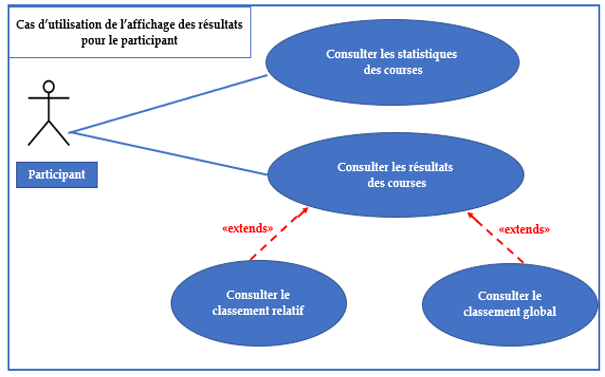
\includegraphics[scale=0.5]{Diagramme_cas_utilisation_consultation_resultats.png}
	   \caption {Le diagramme de cas d’utilisation de l’affichage des résultats pour les participants.}
\end{figure}
\subsection {Diagramme de classes }
\subsubsection{Définition}
Le diagramme de classes est un schéma utilisé en génie logiciel pour présenter les classes et les interfaces des systèmes ainsi que les différentes relations entre celles-ci. Ce diagramme fait partie de la partie statique d'UML car il fait abstraction des aspects temporels et dynamiques.

\subsubsection{Les classes }
Le diagramme de classes du projet est illustré par la figure ci-après :

\begin{figure}
	   \center
	   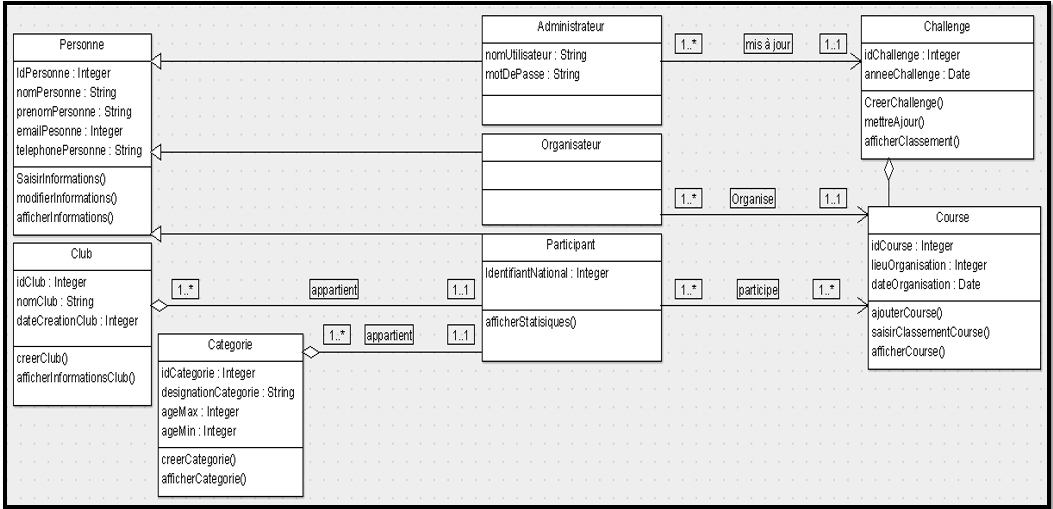
\includegraphics[scale=0.5]{Diagramme_classes.png}
	   \caption {Le diagramme de classes du projet.}
\end{figure}
Le diagramme de classes du projet, figurant dans la capture d’écran précédente est composé de huit classes répertoriées comme suit :
\begin{itemize} 
 	\item La classe Personne qui est une classe abstraite dont héritent les classes Participant, Organisateur et Administrateur. Cette classe possède les attributs suivants : identifiant de la personne, son nom, son prénom, son email et son numéro de téléphone.
 	\item La classe Participant qui est une classe fille de la classe Personne qui possède, en plus des attributs hérités de la classe Personne, un attribut identifiant national qui va permettre de pallier au problème des homonymes dans l’avenir si une migration des données vers une base de données nationale est projetée.
 	\item La classe Administrateur qui est une classe fille de la classe Personne ayant, en plus des attributs hérités de la classe Personne, des attributs d’authentification (nom utilisateur et mot de passe) permettant à l’administrateur de s’authentifier. 
 	\item La classe Organisateur qui hérite ses attributs et ses méthodes de la classe Personne.
 	\item La classe Club : elle représente le club auquel appartient le participant, avec les attributs suivants : nom et la date de création du club.
 	\item La classe Challenge : est une classe qui symbolise les challenges, elle est caractérisée par les attributs : nom, et l’année de création du challenge.
 	\item La classe Course : contient les informations relatives aux courses organisées (la date de l’organisation de la course, le nombre de participants, le lieu d’organisation).
 	\item La classe Catégorie : Comme les participants dans les courses appartiennent à des catégories différentes, il est nécessaire d’implémenter une classe qui stocke les informations inhérentes à chaque catégorie. 
\end{itemize} 
\subsubsection{Les relations entres les classes}
Les différentes classes du diagramme peuvent être liées par des types de relations variées selon la type de relation entre elles et également selon le nombre d’instances générées de chacune d’entre elle lors de l’exécution. Ainsi cet axe est dédié pour détailler ces relations.
\begin{itemize} 
 	\item Les classes Participant, Organisateur et Administrateur sont des classes filles de la classe Personne, c’est-à-dire qu’elles héritent des méthodes et des attributs de celle-ci. Il reste à préciser que les méthodes seront surchargées ou redéfinies selon chaque classe.
 	\item La classe Club et la Classe Participant sont liées par une relation d’agrégation c’est-à-dire que plusieurs participants appartiennent à un club et une personne adhère à un seul Club.
 	\item La classe Participante est liée à la classe course par une relation d’association, en effet un participant peut participer à plusieurs courses et une course est ouverte à plusieurs personnes.
 	\item Une Course doit être insérer dans un seul challenge, vu que la classe Course et Challenge sont liées par une relation d’association avec les cardinalités 1..1 du coté de la course.
 	\item Un participant appartient à une et une seule catégorie, alors qu’une catégorie peut contenir plusieurs participants. 
	\item Une course est organisée par un seul Organisateur et un organisateur peut organiser plusieurs courses.
 	\item Un administrateur peur mettre à jour plusieurs Challenge, et un Challenge est obligatoirement par un seul administrateur.
 	\item Les résultats d’une course figurent dans un seul fichier Challenge et un challenge peut contenir plusieurs courses. 
\end{itemize} 


\subsection {Le diagramme d’activités  }
\subsubsection{Définition}
Les diagrammes d'activités permettent de mettre l'accent sur les traitements. Ils sont donc particulièrement adaptés à la modélisation du cheminement et de contrôle des flots de données. 
\subsubsection{Le diagramme d'activité du projet}
\begin{figure}
	   \center
	   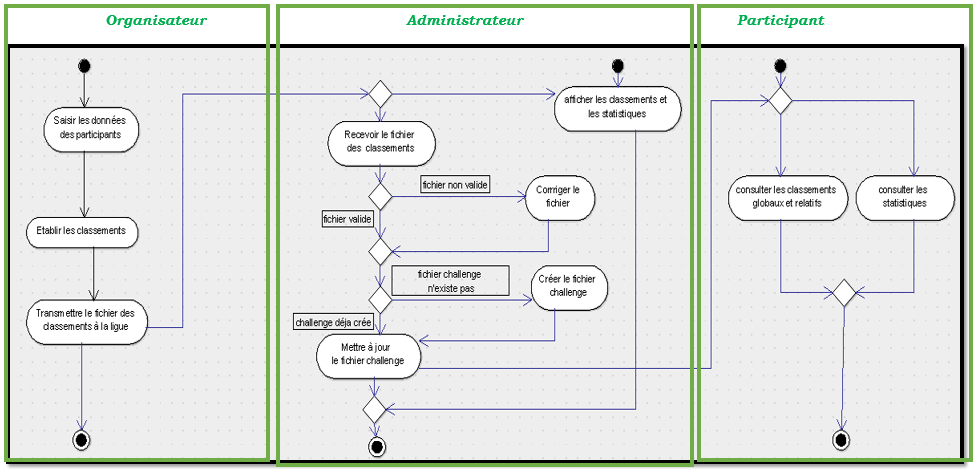
\includegraphics[scale=0.5]{Diagramme_activites.png}
	   \caption {Le diagramme d’activités du projet}
\end{figure}

Le diagramme illustré dans la figure ci-dessous montre le diagramme d’activités du projet. En effet, il représente les événements déclencheurs des différents processus. Egalement, il illustre les différentes tâches exécutées d’une manière séquentielle. 
\newpage
\chapter{Réalisation du projet}
Ce chapitre est l’occasion pour présenter les différents langage et outils utilisés pour réaliser le projet. Egalement, la mise en avant des différentes interfaces mises en œuvres pour l’exécution des différentes fonctionnalités. Enfin les tests effectués pour s’assurer du bon fonctionnement de logiciel.

\newpage
\section {Réalisation du projet }
\subsection {Langages et outils utilisé  }
\subsubsection {Langage R  }



\subsubsection {Serveur Shiny}

\subsubsection {Fichiers Excel}




	
	
	\end{document}